\documentclass[11pt,t]{beamer}
% xcolor and define colors -------------------------
\usepackage{xcolor}

% https://www.viget.com/articles/color-contrast/
\definecolor{purple}{HTML}{695693}
\definecolor{navy}{HTML}{567293}
\definecolor{ruby}{HTML}{9a2515}
\definecolor{alice}{HTML}{107895}
\definecolor{daisy}{HTML}{EBC944}
\definecolor{coral}{HTML}{F26D21}
\definecolor{kelly}{HTML}{829356}
\definecolor{cranberry}{HTML}{E64173}
\definecolor{jet}{HTML}{131516}
\definecolor{asher}{HTML}{555F61}
\definecolor{slate}{HTML}{314F4F}

% Main theme colors
\definecolor{accent}{HTML}{107895}
\definecolor{accent2}{HTML}{9a2515}

\newcommand\navy[1]{{\color{navy}#1}}
\newcommand\purple[1]{{\color{purple}#1}}
\newcommand\kelly[1]{{\color{kelly}#1}}
\newcommand\ruby[1]{{\color{ruby}#1}}
\newcommand\alice[1]{{\color{alice}#1}}
\newcommand\daisy[1]{{\color{daisy}#1}}
\newcommand\coral[1]{{\color{coral}#1}}
\newcommand\cranberry[1]{{\color{cranberry}#1}}
\newcommand\slate[1]{{\color{slate}#1}}
\newcommand\jet[1]{{\color{jet}#1}}
\newcommand\asher[1]{{\color{asher}#1}}

\newcommand\bgNavy[1]{{\colorbox{navy!80!white}{\textcolor{white}{#1}}}}
\newcommand\bgPurple[1]{{\colorbox{purple!80!white}{\textcolor{white}{#1}}}}
\newcommand\bgKelly[1]{{\colorbox{kelly!80!white}{\textcolor{white}{#1}}}}
\newcommand\bgRuby[1]{{\colorbox{ruby!80!white}{\textcolor{white}{#1}}}}
\newcommand\bgAlice[1]{{\colorbox{alice!80!white}{\textcolor{white}{#1}}}}
\newcommand\bgDaisy[1]{{\colorbox{daisy!80!white}{\textcolor{white}{#1}}}}
\newcommand\bgCoral[1]{{\colorbox{coral!80!white}{\textcolor{white}{#1}}}}
\newcommand\bgCranberry[1]{{\colorbox{cranberry!80!white}{\textcolor{white}{#1}}}}


% Beamer Options -------------------------------------

% Background
\setbeamercolor{background canvas}{bg = white}

% Change text margins
\setbeamersize{text margin left = 15pt, text margin right = 15pt} 

% \alert
\setbeamercolor{alerted text}{fg = accent2}

% Frame title
\setbeamercolor{frametitle}{bg = white, fg = jet}
\setbeamercolor{framesubtitle}{bg = white, fg = accent}
\setbeamerfont{framesubtitle}{size = \small, shape = \itshape}

% Block
\setbeamercolor{block title}{fg = white, bg = accent2}
\setbeamercolor{block body}{fg = jet, bg = jet!10!white}

% Title page
\setbeamercolor{title}{fg = jet}
\setbeamercolor{subtitle}{fg = accent}

%% Custom \maketitle and \titlepage
\setbeamertemplate{title page}
{
    %\begin{centering}
        \vspace{20mm}
        {\Large \usebeamerfont{title}\usebeamercolor[fg]{title}\inserttitle}\\ \vskip0.25em%
        \ifx\insertsubtitle\@empty%
        \else%
          {\usebeamerfont{subtitle}\usebeamercolor[fg]{subtitle}\insertsubtitle\par}%
        \fi% 
        {\vspace{10mm}\insertauthor}\\
        {\color{asher}\small{\insertdate}}\\
    %\end{centering}
}

% Table of Contents
\setbeamercolor{section in toc}{fg = accent!70!jet}
\setbeamercolor{subsection in toc}{fg = jet}

% Button 
\setbeamercolor{button}{bg = accent}

% Remove navigation symbols
\setbeamertemplate{navigation symbols}{}

% Optional: page numbers at bottom
\addtobeamertemplate{navigation symbols}{}{%
    \usebeamerfont{footline}%
    \hspace{1em}%
    \alice{\insertframenumber/\inserttotalframenumber}
    \vspace*{1.5mm}
}


% Table and Figure captions
\setbeamercolor{caption}{fg=jet!70!white}
\setbeamercolor{caption name}{fg=jet}
\setbeamerfont{caption name}{shape = \itshape}

% Bullet points

%% Fix left-margins
\settowidth{\leftmargini}{\usebeamertemplate{itemize item}}
\addtolength{\leftmargini}{\labelsep}

%% enumerate item color
\setbeamercolor{enumerate item}{fg = accent}
\setbeamerfont{enumerate item}{size = \small}
\setbeamertemplate{enumerate item}{\insertenumlabel.}

%% enumerate subitem color
\setbeamercolor{enumerate subitem}{fg = accent!60!white}
\setbeamerfont{enumerate subitem}{size = \small}
\setbeamertemplate{enumerate subitem}{\insertenumlabel.}

%% itemize
\setbeamercolor{itemize item}{fg = accent!70!white}
\setbeamerfont{itemize item}{size = \small}
\setbeamertemplate{itemize item}[circle]

%% right arrow for subitems
\setbeamercolor{itemize subitem}{fg = accent!60!white}
\setbeamerfont{itemize subitem}{size = \small}
\setbeamertemplate{itemize subitem}{$\rightarrow$}

\setbeamertemplate{itemize subsubitem}[square]
\setbeamercolor{itemize subsubitem}{fg = jet}
\setbeamerfont{itemize subsubitem}{size = \small}

% References

%% Bibliography Font, roughly matching aea
\setbeamerfont{bibliography item}{size = \footnotesize}
\setbeamerfont{bibliography entry author}{size = \footnotesize, series = \bfseries}
\setbeamerfont{bibliography entry title}{size = \footnotesize}
\setbeamerfont{bibliography entry location}{size = \footnotesize, shape = \itshape}
\setbeamerfont{bibliography entry note}{size = \footnotesize}

\setbeamercolor{bibliography item}{fg = jet}
\setbeamercolor{bibliography entry author}{fg = accent!60!jet}
\setbeamercolor{bibliography entry title}{fg = jet}
\setbeamercolor{bibliography entry location}{fg = jet}
\setbeamercolor{bibliography entry note}{fg = jet}

%% Remove bibliography symbol in slides
\setbeamertemplate{bibliography item}{}





% Links ----------------------------------------------

\usepackage{hyperref}
\hypersetup{
  colorlinks = true,
  linkcolor = accent2,
  filecolor = accent2,
  urlcolor = accent2,
  citecolor = accent2,
}


% Line spacing --------------------------------------
\usepackage{setspace}
% \setdisplayskipstretch{2}
\setstretch{1.3}


% \begin{columns} -----------------------------------
\usepackage{multicol}


% Fonts ---------------------------------------------
% Beamer Option to use custom fonts
\usefonttheme{professionalfonts}

% \usepackage[utopia, smallerops, varg]{newtxmath}
% \usepackage{utopia}
\usepackage[sfdefault,light]{roboto}

% Small adjustments to text kerning
\usepackage{microtype}



% Remove annoying over-full box warnings -----------
\vfuzz2pt 
\hfuzz2pt


% Table of Contents with Sections
\setbeamerfont{myTOC}{series=\bfseries, size=\Large}
\AtBeginSection[]{
        \frame{
            \frametitle{Roadmap}
            \tableofcontents[current]   
        }
    }


% References ----------------------------------------
\usepackage[
    citestyle= authoryear,
    style = authoryear,
    natbib = true, 
    backend = biber
]{biblatex}

% Smaller font-size for references
\renewcommand*{\bibfont}{\small}

% Remove "In:"
\renewbibmacro{in:}{}

% Color citations for slides
\newenvironment{citecolor}
    {\footnotesize\begin{color}{accent2}}
    {\end{color}}

\newcommand{\citetcolor}[1]{{\footnotesize\textcolor{gray}{\citet{#1}}}}
\newcommand{\citepcolor}[1]{{\footnotesize\textcolor{gray}{\citep{#1}}}}

% Tables -------------------------------------------
% Tables too big
% \begin{adjustbox}{width = 1.2\textwidth, center}
\usepackage{adjustbox}
\usepackage{array}
\usepackage{threeparttable, booktabs, adjustbox}
    
% Fix \input with tables
% \input fails when \\ is at end of external .tex file

\makeatletter
\let\input\@@input
\makeatother

% Tables too narrow
% \begin{tabularx}{\linewidth}{cols}
% col-types: X - center, L - left, R -right
% Relative scale: >{\hsize=.8\hsize}X/L/R
\usepackage{tabularx}
\newcolumntype{L}{>{\raggedright\arraybackslash}X}
\newcolumntype{R}{>{\raggedleft\arraybackslash}X}
\newcolumntype{C}{>{\centering\arraybackslash}X}

% Figures

% \imageframe{img_name} -----------------------------
% from https://github.com/mattjetwell/cousteau
\newcommand{\imageframe}[1]{%
    \begin{frame}[plain]
        \begin{tikzpicture}[remember picture, overlay]
            \node[at = (current page.center), xshift = 0cm] (cover) {%
                \includegraphics[keepaspectratio, width=\paperwidth, height=\paperheight]{#1}
            };
        \end{tikzpicture}
    \end{frame}%
}

% subfigures
\usepackage{subfigure}

% Strikeout text
\usepackage{cancel}

% Highlight slide -----------------------------------
% \begin{transitionframe} Text \end{transitionframe}
% from paulgp's beamer tips
\newenvironment{transitionframe}{
    \setbeamercolor{background canvas}{bg=accent!60!black}
    \begin{frame}\color{accent!10!white}\LARGE\centering
}{
    \end{frame}
}


% Table Highlighting --------------------------------
% Create top-left and bottom-right markets in tabular cells with a unique matching id and these commands will outline those cells
\usepackage[beamer,customcolors]{hf-tikz}
\usetikzlibrary{calc,fit,shapes.misc,backgrounds}
\usepackage{pgfplots}
\pgfplotsset{compat = newest}
\usetikzlibrary{positioning, arrows.meta}
\usepgfplotslibrary{fillbetween}

% halo around text
%https://tex.stackexchange.com/questions/18472/tikz-halo-around-text
\usepackage[outline]{contour} 
\contourlength{1.2pt}
\tikzset{
  contour text/.style={node contents={\contour{white}{#1}}},
  halo text node/.style={circle, draw, pattern=north east lines}
}


\def\arraystretch{0.75}

% To set the hypothesis highlighting boxes red.
\newcommand\marktopleft[1]{%
    \tikz[overlay,remember picture] 
        \node (marker-#1-a) at (0,1.5ex) {};%
}
\newcommand\markbottomright[1]{%
    \tikz[overlay,remember picture] 
        \node (marker-#1-b) at (0,0) {};%
    \tikz[accent!80!jet, ultra thick, overlay, remember picture, inner sep=4pt]
        \node[draw, rectangle, fit=(marker-#1-a.center) (marker-#1-b.center)] {};%
}


\author{Michael Karas}
\title{Lecture 6  - Producer Theory}
\subtitle{ECON 3070 - Intermediate Microeconomic Theory}
\date{February X, 2025}

\begin{document}

\begin{frame}
  \titlepage
\end{frame}

\begin{frame}{Overview}
  In the next lecture, we begin discussing production functions.
  
  \bigskip
  \begin{itemize}
    \item How do we represent, both graphically and numerically, the relationship between inputs and output?

    \item What role does technology play in production?

    \item What is the relationship between different mixes of inputs, and the level of output?
  \end{itemize}
\end{frame}

\begin{frame}{Inputs and the Production Function}
  Production means transforming things such as labor, materials, and energy, into finished products or services.
  
  \bigskip
  \begin{itemize}
    \item \textbf{Inputs} are the capital, labor, materials, and energy used to produce \textbf{output}, or final goods and services.

    \item A \textbf{production function} relates the amount of every input used to the amount of output that will be produced.
  \end{itemize}

  \pause\bigskip
  \begin{center}
    \emph{All of the following slides is going to seem really similar to the consumer setting. The skills you have already learned will help with this a lot}
  \end{center}
\end{frame}

\begin{frame}{Production Functions}
  Production functions take the form
  \begin{equation*}
    Q=f(L,K)
  \end{equation*}
  
  \bigskip
  \begin{itemize}
    \item Where $Q$ is the quantity of output, $L$ and $K$ are the quantity of labor and capital used, respectively.

  \end{itemize}
  
  \bigskip
  This relation tells us that the quantity of output is a function of the amount of inputs used.
\end{frame}

\begin{frame}{Production Functions}
  Output is not always simply a function of labor and capital.
  
  \bigskip
  \begin{itemize}
    \item It could also be a function of natural resources, such as oil or diamonds, or of raw materials such as wood and computer chips.

    \item Even labor can be divided up by type (for example, high- and low-skilled labor).
  \end{itemize}
\end{frame}

\begin{frame}{Examples of Production Functions}
  Example 1: Lawn Care Company

  \begin{itemize}
    \item $Q(K,L) = 1/2 * min(K,L)$
    \item $K$ is number of lawn mowers, $L$ is number of workers, $Q$ is number of lawns mowed per hour.
    \item Each worker needs exactly 1 lawn mower.
  \end{itemize}

  \bigskip
  Example 2: Grocery Store Checkout

  \begin{itemize}
    \item $Q(K,L) = 10K + 15L$
    \item $K$ is number of self-checkout machines, $L$ is the number of cashiers, and $Q$ is customers served per hour.
    \item Cashiers and self-checkout machines are substitutes.
  \end{itemize}
\end{frame}

\begin{frame}{Examples of Production Functions}
  Example 3: Dog Grooming Company

  \begin{itemize}
    \item $Q(K,L) = 10K - K^2 + 8L - L^2 + KL$
    \item $Q$ is number of dogs groomed per day, $K$ is number of dog grooming stations, and L is number of dog groomers.
    \item More workers and more stations mean more dogs groomed, but eventually the grooming room gets too crowded ($-L^2$).
  \end{itemize}
\end{frame}

\begin{frame}{Production Functions}
  Production functions tell us the maximum output that a firm can produce from a given combination of inputs.
  
  \bigskip
  But output could be lower than what is technically feasible. Why?
  
  \bigskip\pause
  \begin{itemize}

    \item All points on or below the production function make up the firm's \textbf{production set}.

    \item Therefore, we say that any point on the production function is considered \textbf{technologically efficient}.

    \item Any point below the production function is \textbf{technologically inefficient}. 
  \end{itemize}
\end{frame}

\begin{frame}{Production Functions}
  Below is a graphical representation of a production function $Q=f(L)$.

  \begin{figure}
    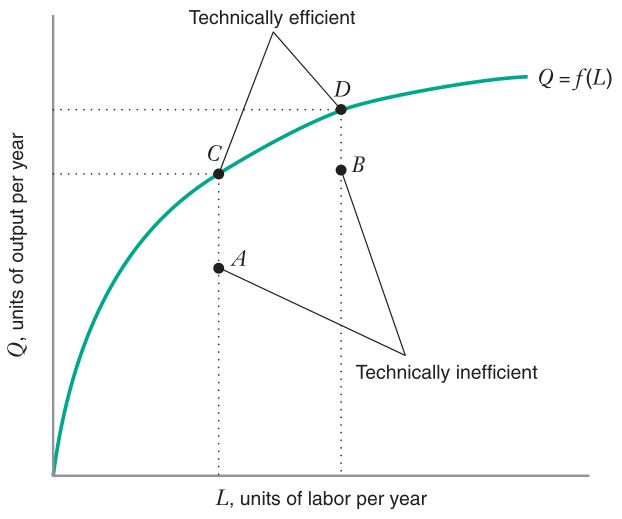
\includegraphics[width=0.7\linewidth]{figures/fig6_1.jpg}
  \end{figure}
\end{frame}

\begin{frame}{Marginal and Average Product}
  For now, we will consider production functions with only one input; labor.
  
  \bigskip
  \begin{itemize}
    \item Firms consider the \textbf{marginal product} of each of their inputs when maximizing profit.

    \item The marginal product of labor measures how output changes if we add an additional unit of labor.

    \begin{equation*}
      MP_L =\frac{\text{change in total product}}{\text{change in quantity of labor}}= \frac{\Delta Q}{\Delta L} = \frac{\partial Q}{\partial L}
    \end{equation*}
  \end{itemize}
\end{frame}

\begin{frame}{Marginal and Average Product}
  \textbf{Increasing marginal returns to labor} - $MP_L$ is increasing
  \bigskip
  \begin{itemize}
    \item Each additional unit of labor produces more output than the previous unit
  \end{itemize}

  \pause\bigskip
  \textbf{Diminishing marginal returns to labor} -$MP_L$ is decreasing.

  \bigskip
  \textbf{Diminishing total returns to labor} - additional labor results in lower \textit{total} output.
\end{frame}

\begin{frame}{Marginal and Average Product}
  Below is a production function with labor as it's only input.
  \begin{figure}
    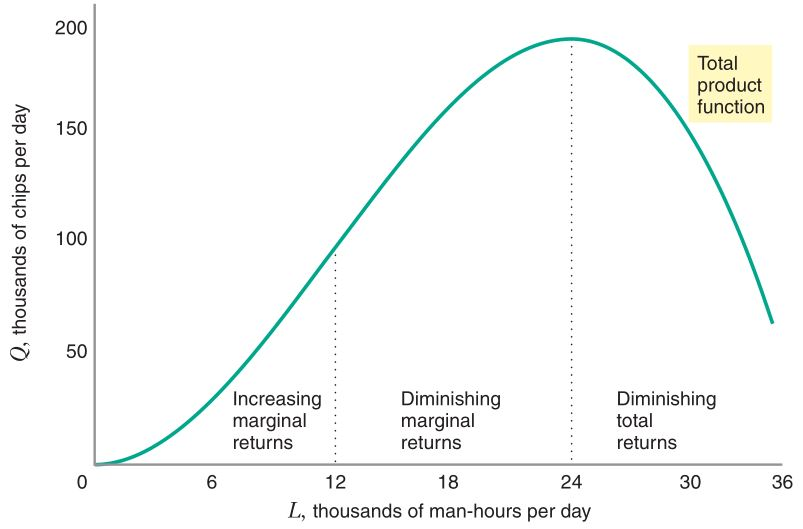
\includegraphics[width=0.8\linewidth]{figures/fig6_2.jpg}
  \end{figure}
\end{frame}

\begin{frame}{Marginal and Average Product}
  \bgCranberry{Try It Yourself}
  
  \bigskip
  Suppose a firm uses only labor in the production of it's good, and that the firm's production function is $Q(L) = 4\sqrt{L}$. What is the firm's marginal product of labor if $L=4$?

  
\end{frame}

\begin{frame}{Marginal and Average Product}
  In reality, most production processes experience diminishing marginal returns eventually.
  
  \bigskip
  \begin{itemize}
    \item This is what economists call the \textbf{law of diminishing marginal returns}.
  \end{itemize}

  \pause\bigskip
  Another measure of productivity commonly discussed is \textbf{average product}. For example, the average product of labor is given by:
  
  \begin{equation*}
    AP_L = \frac{\text{total product}}{\text{quantity of labor}} = \frac{Q}{L}
  \end{equation*}
\end{frame}

\begin{frame}{Marginal and Average Product}
  Here is a numerical example of calculating marginal and average product:

  \begin{center}
    \begin{spacing}{1.9}
      \begin{tabular}{ | l | l | l | l |}
        \hline
        $L$ & $Q$ & $MP_L$ & $AP_L$ \\ \hline
        0 & 0  & - & - \\ \hline
        2 & 12 &   &   \\ \hline
        4 & 20 &   &   \\ \hline
        6 & 24 &   &   \\ \hline
        8 & 24 &   &   \\
        \hline
      \end{tabular}
    \end{spacing}
  \end{center}
\end{frame}

\begin{frame}
  \bgCranberry{Try It Yourself}
  
  \bigskip
  Given the following production table, find the marginal product of labor and the average product of labor
  \begin{center}
    \begin{spacing}{1.9}
      \begin{tabular}{ | l | l | l | l |}
        \hline
        $L$ & $Q$ & $MP_L$ & $AP_L$ \\ \hline
        0  & 0  & - & - \\ \hline
        6  & 15 &   &   \\ \hline
        9  & 24 &   &   \\ \hline
        12 & 30 &   &   \\ \hline
        15 & 33 &   &   \\
        \hline
      \end{tabular}
    \end{spacing}
  \end{center}
\end{frame}

\begin{frame}{Relationship Between Marginal and Average Product}
  There is a systematic relationship between average product and marginal product.
  
  \bigskip
  \begin{itemize}
    \item If $AP_L$ increases in $L$, then $MP_L > AP_L$.
    \begin{itemize}
      \item If your last unit of labor produced more than the average, then your average increases
    \end{itemize}

    \pause
    \item If $AP_L$ decreases in $L$, then $MP_L < AP_L$.
    \begin{itemize}
      \item If your last unit of labor produced less than the average, then your average decreases
    \end{itemize}

    \pause
    \item $MP_L$ intersects $AP_L$ at the maximum of $AP_L$.
  \end{itemize}
\end{frame}

\begin{frame}{Relationship Between Marginal and Average Product}
  As an analogy, consider calculating the average grade on an exam. Suppose the average is 80\%.

  \bigskip
  \begin{itemize}
    \item If one additional student takes the exam late, and they score 70\%...

    \item Then the \textit{marginal} grade is lower than the average, and the \textit{average} falls.

    \item On the other hand, if the \textit{marginal} grade is 90\%, then the \textit{average} rises.
  \end{itemize}
\end{frame}

\begin{frame}{Relationship Between Marginal and Average Product}
  \begin{figure}
    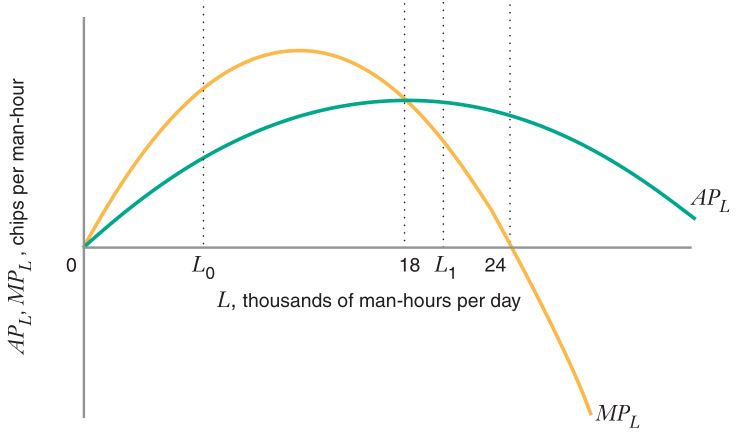
\includegraphics[width=\linewidth]{figures/fig6_4b.jpg}
  \end{figure}
\end{frame}

\begin{frame}{Production with Multiple Inputs}
  Now, let's consider a firm that uses two goods, labor (L) and capital (K).
  
  \begin{itemize}
    \item Below is a table of output, similar to the table we saw earlier, but with two inputs:
  \end{itemize}

  \begin{figure}
    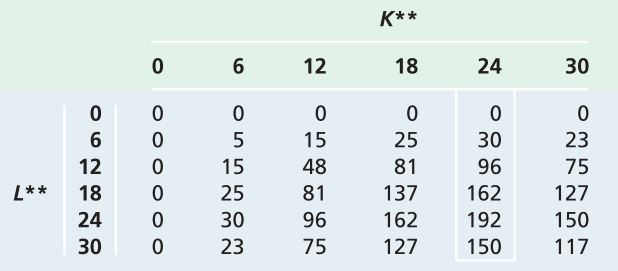
\includegraphics[width=\linewidth]{figures/table6_3.jpg}
  \end{figure}
\end{frame}

\begin{frame}
  \begin{center}\begin{figure}
    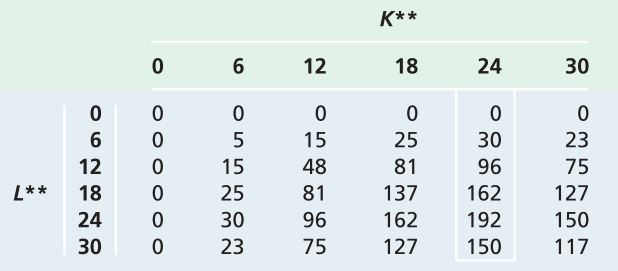
\includegraphics[width=0.9\linewidth]{figures/table6_3.jpg}
  \end{figure}\end{center}

  \begin{itemize}
    \item As K increases, for any given level of L, output first increases and then decreases. \pause The same is true for L.

    \item This illustrates the \textbf{law of diminishing marginal product} for both inputs.
  \end{itemize}

  
\end{frame}

\begin{frame}{Marginal Product}
  Suppose we want to know how $MP_L$ changes as we increase L.
  
  \bigskip
  \begin{itemize}
    \item Well, that depends on what the level of capital is. 

    \only<1>{
      \begin{itemize}
        \item For example, if you had one coffee machine, adding a bunch of workers produces no extra coffee
      \end{itemize}
    }
  \end{itemize}

  \pause\bigskip
  In order to find the marginal product of one input, we have to hold the other input fixed. For example,
  \begin{align*}
    MP_L & =\frac{\text{\textit{change} in quantity of output }Q}{\text{\textit{change} in quantity of labor }L} \Biggr\vert_{K \text{ is held constant}} \\
    & =\frac{\Delta Q}{\Delta L}\Biggr\vert_{K \text{ is held constant}} = \frac{\partial Q}{\partial L}
  \end{align*}
\end{frame}

\begin{frame}
  \bgCranberry{Try It Yourself}
  
  \bigskip
  Suppose a tutoring company has the production function $Q(K,L) = 8K - K^2 + 4L - \tfrac{1}{2} L^2 + KL$. What is the marginal product of capital for this company?
\end{frame}

\begin{frame}{Isoquants}
  When thinking about consumers, we had a concept of indifference curves. Bundles of goods that created the same level of utility. 
  
  \bigskip\pause
  For producers, we think of \textbf{isoquants} which are bundles of inputs that create the same level of output

  \bigskip\pause
  \begin{itemize}
    \item A graph of isoquants and a graph of indifference curves are both just `contour plots' of their respective functions.

    \item ``Iso" is Greek for same. ``quant" is short for quantity.
  \end{itemize}
\end{frame}

\begin{frame}{Isoquants}
  Below is a plot of a production function with countour lines (isoquants) drawn onto it.

  \begin{figure}
    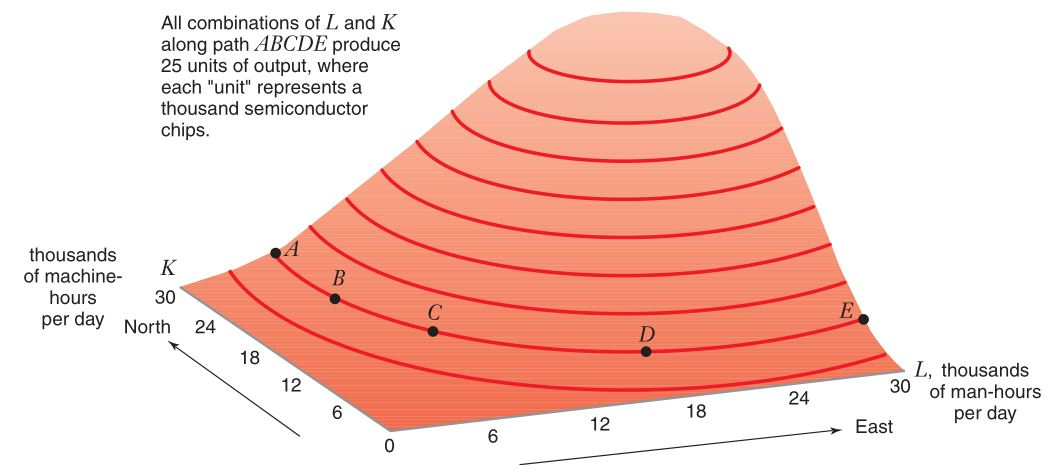
\includegraphics[width=\linewidth]{figures/fig6_6.jpg}
  \end{figure}
\end{frame}

\begin{frame}{Isoquants}
  And this is a subset of those isoquants plotted in two dimensions.
  
  \begin{figure}
    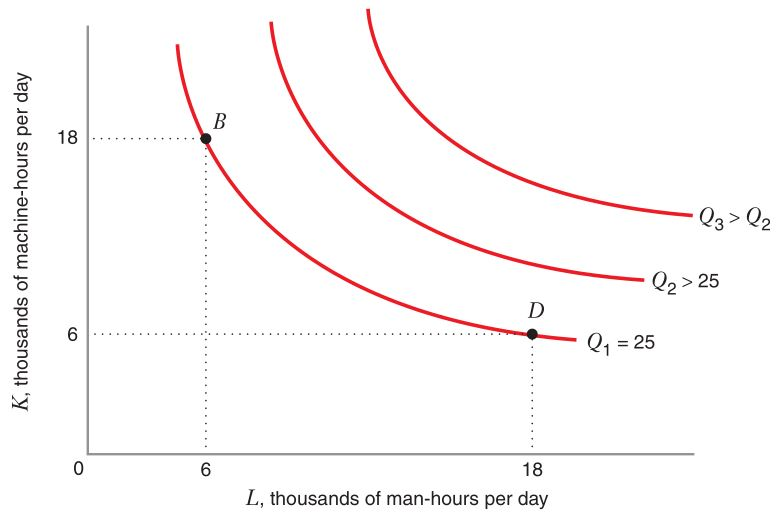
\includegraphics[width=0.9\linewidth]{figures/fig6_8.jpg}
  \end{figure}
\end{frame}

\begin{frame}{Marginal Rate of Technical Substitution}
  The isoquants illustrate the tradeoff that can be made in production between two inputs (holding quantity of output constant)...
  
  \bigskip
  \begin{itemize}
    \item The slope of these isoquants tells us the rate at which inputs can be substituted, or the \textbf{marginal rate of technical substitution}. We call this $MRTS$ for short (similar to $MRS$!).
  \end{itemize}

  \pause\bigskip
  For example, the $MRTS_{L,K}$ tells us that if we want to keep output \emph{constant}, then a one-unit \textit{decrease} in labor can be replaced with $MRTS_{L, K}$ additional units of capital.
\end{frame}

\begin{frame}{Marginal Rate of Technical Substitution}
  Below is a single isoquant for a production function. The slope of this isoquant at any given point is the $MRTS_{L,K}$.
  
  \begin{figure}
    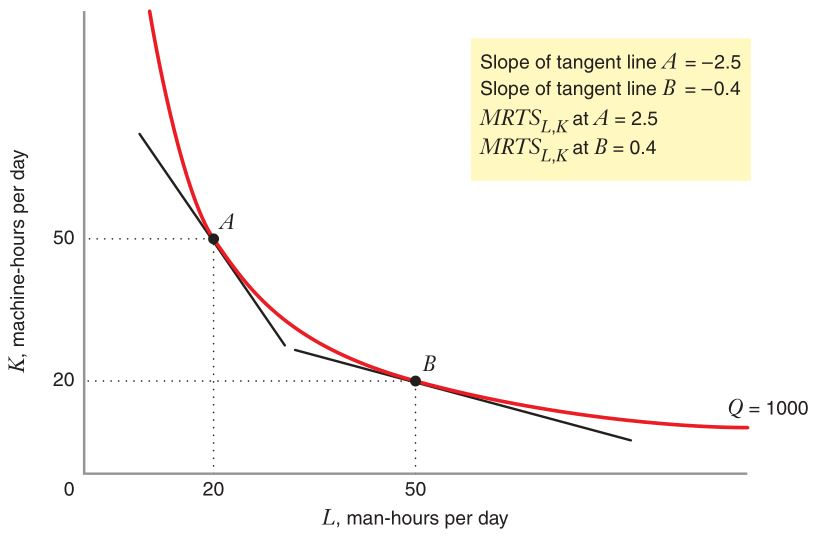
\includegraphics[width=0.8\linewidth]{figures/fig6_10.jpg}
  \end{figure}
\end{frame}

\begin{frame}{Marginal Rate of Technical Substitution}
  Note that as we move along the isoquant to the right, the curve becomes flatter.
  
  \bigskip
  \begin{itemize}
    \item This is because for every additional unit of capital you give up, you must compensate with more and more labor.

    \item This is known as the \textbf{diminishing marginal rate of technical substitution}.
  \end{itemize}
\end{frame}

\begin{frame}{Marginal Rate of Technical Substitution}
  We can show mathematically that the MRTS is the slope of the isoquant with a little bit of math:
  
  $$
    \Delta Q = (\Delta K)(MP_K) + (\Delta L)(MP_L)
  $$

  \pause\bigskip
  In order to stay on the same isoquant, $\Delta Q = 0$.

  \vspace*{-10mm}
  \begin{align*} 
    &\quad 0 = (\Delta K)(MP_K) + (\Delta L)(MP_L) \\
    &\implies (\Delta K)(MP_K) = - (\Delta L)(MP_L) \\\pause
    &\implies -\frac{\Delta K}{\Delta L} = \frac{MP_L}{MP_K} \\
    &\implies \frac{MP_L}{MP_K} = MRTS_{L,K}
  \end{align*}
\end{frame}

\begin{frame}
  \bgCranberry{Try It Yourself}
  
  \bigskip
  Suppose a firm has the production function $Q(K,L) = 20K-2K^2 + 14L - 2L^2$. Find the firm's $MRTS_{L,K}$ when $L=2$ and $K=3$.
\end{frame}

\begin{frame}{Economic Region of Production}
  In theory, there could be points where a firm's $MRTS_{L,K}$ is negative, but a firm would never produce at these points.
  
  \bigskip
  \begin{itemize}
    \item Usually this is because there is another input that is fixed (e.g. building space) that suffers from diminishing returns
    
    \pause
    \item These are called \textbf{uneconomic regions of production}.
  \end{itemize}

  \bigskip
  A firm would never produce in this region because they could choose an input combination with both less labor and less capital that produces the same quantity of output.
\end{frame}

\begin{frame}{Economic Region of Production}
  This graph illustrates economic and uneconomic regions of production. Note that points A and E produce the same amount of output using the same amount of capital, but A uses substantially more labor.

  \begin{figure}
    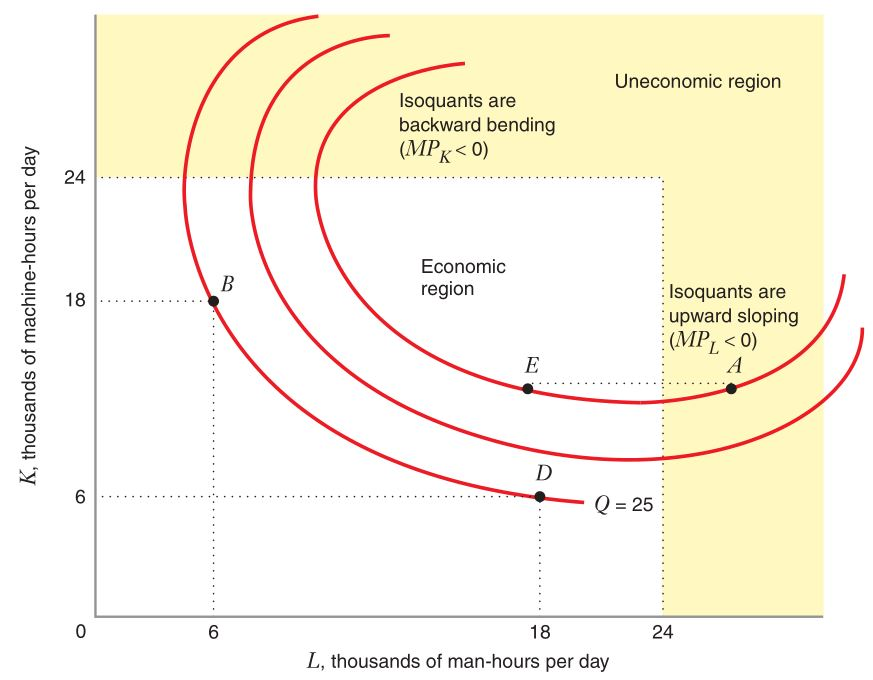
\includegraphics[width = 0.6\linewidth]{figures/fig6_9.jpg}
  \end{figure}
\end{frame}

\begin{frame}{Substitutablity of Inputs}
  For some firms, labor and capital are easily substitutable.
  
  \bigskip
  \begin{itemize}
    \item Think of the example of cashiers and self-checkout machines at the grocery store.

    \item These firms can more easily switch between high capital-labor ratio and low capital-labor ratio, depending on their needs
  \end{itemize}
  
  \pause\bigskip
  But for other firms, labor and capital cannot be easily substituted.

  \bigskip
  \begin{itemize}
    \item Such as in a lawn care company. You could substitute a lawnmower for workers who just pluck at the grass with their hands...
  \end{itemize}
\end{frame}

\begin{frame}{Substitutablity of Inputs}
  The isoquants for the grocery store might look similar to these ones, where labor and capital are easily interchanged at some ratio (lets say 2 self-checkout machines to 1 cashier).

  \begin{figure}
    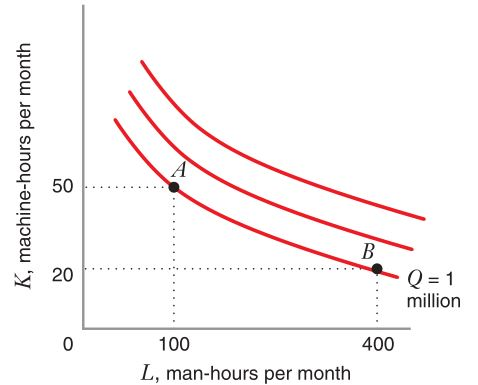
\includegraphics[width=0.6\linewidth]{figures/fig6_11b.jpg}
  \end{figure}
\end{frame}

\begin{frame}{Substitutablity of Inputs}
  The isoquants for a lawn care company might look like these ones, where, if we move away from the corners (lets say a 1-to-1 ratio of workers and lawn mowers), it takes a very large amount of labor to make up for a lost unit of capital, and vice versa.

  \begin{figure}
    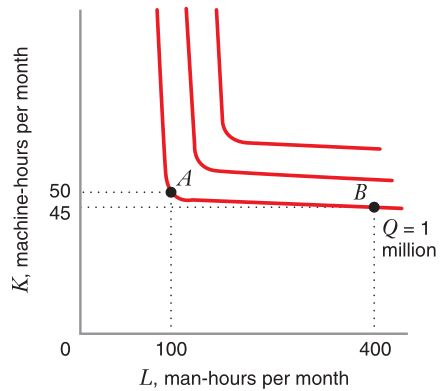
\includegraphics[width=0.5\linewidth]{figures/fig6_11a.jpg}
  \end{figure}
\end{frame}

\begin{frame}{The three \xcancel{utility} production functions in this class}
    There are three kinds of production functions we will give you in this course. 
    
    \bigskip\bigskip
    If you want to do well in this class, you should practice these three functions a bunch \emph{(calculate MRTS, draw isoquant curves, and later on calculate supply curves for $K$ and $L$)}
\end{frame}

\begin{frame}{Three Production Functions}
  \begin{enumerate}
    \item \textbf{Cobb-Douglas}: $Q(K,L) = K^\alpha L^\beta$
    
    \item \textbf{Perfect Subsitutes}: $Q(K,L) = aK + bL$
    
    \item \textbf{Perfect Complements}: $Q(K,L) = \min\big(aK, bL\big)$
  \end{enumerate}
  
  \pause\bigskip
  Which functions represent the above two examples (lawncare and grocery store checkout)?
\end{frame}

\begin{frame}{Elasticity of Substitution}
  We can use the elasticity of substitution to more accurately describe the substitution opportunities in a firm's production function.
  
  \bigskip
  \begin{itemize}
    \item The \textbf{elasticity of substitution} measures how quickly the marginal rate of technical substitution changes as we move along the isoquant.
    
    \begin{align*}
      \sigma & = \frac{\text{\textit{percentage change} in capital-labor ratio}}{\text{\textit{percentage change} in }MRTS_{L,K}} \\
      & = \frac{\% \Delta \frac{K}{L}}{\% \Delta MRTS_{L,K}}
    \end{align*}
  \end{itemize}
\end{frame}

\begin{frame}{Elasticity of Substitution}
  \begin{figure}
    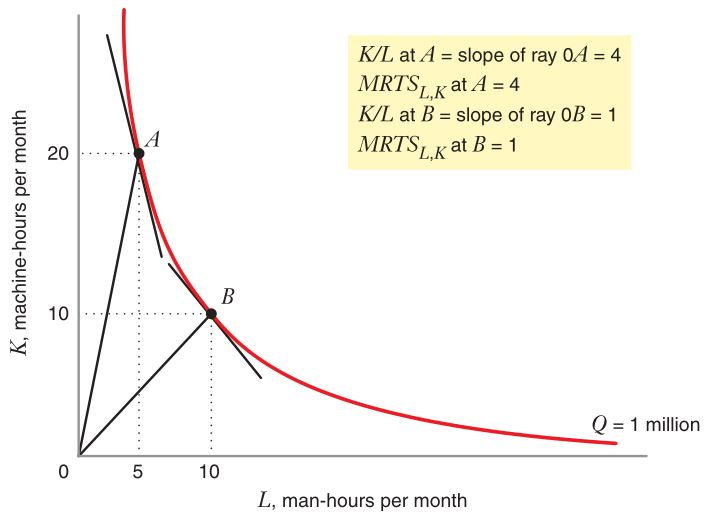
\includegraphics[width=240px]{figures/fig6_12.jpg}
  \end{figure}
\end{frame}

\begin{frame}{Elasticity of Substitution}
  What does the elasticity of substition tell us?
  
  \bigskip
  \begin{itemize}
    \item If $\sigma$ is close to zero, there is little opportunity to substitute between inputs.

    \item If $\sigma$ is large, there is greater opportunity to substitute between inputs.
  \end{itemize}
\end{frame}

\begin{frame}{Elasticity of Substitution}
  \begin{figure}
    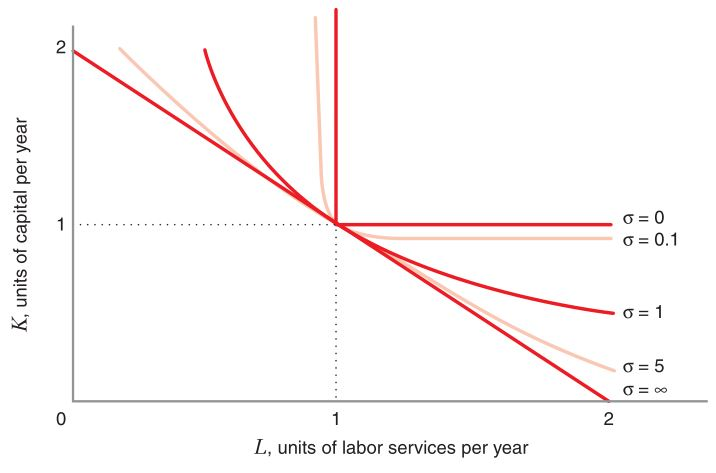
\includegraphics[width=\linewidth]{figures/fig6_17.jpg}
  \end{figure}
\end{frame}

\begin{frame}{Returns to Scale}
  We looked at how output responds when a firm increases the quantity of some input, holding all others fixed.
  
  \begin{itemize}
    \item But what about when a firm increases all input quantities?
  \end{itemize}
  
  \pause\bigskip
  \textbf{Returns to scale} tell us the percentage increase in output when a firm increases all of its inputs by a given percentage amount. Mathematically,
  \begin{equation*}
    \text{Returns to scale} = \frac{\% \Delta \text{ quantity of output}}{\% \Delta \text{ quantity of \textit{all} inputs}}
  \end{equation*}
\end{frame}

\begin{frame}{Returns to Scale}
  A production function is said to exhibit \textbf{constant returns to scale} if multiplying both inputs by a given factor increases output by the same factor. That is...
  
  $$
    Q(\phi K, \phi L) = \phi Q(K,L)
  $$
  
  \bigskip\pause
  \begin{itemize}
    \item Suppose $\phi$ equals 2. Then if we double the amount of both inputs used, our output will double.
  \end{itemize}
\end{frame}

\begin{frame}{Returns to Scale}
  
  \textbf{Increasing returns to scale} implies that scaling both inputs by some factor increases output by \textit{more} than that factor.

  $$
    Q(\phi K, \phi L) > \phi Q(K,L)
  $$

  \bigskip
  \textbf{Decreasing returns to scale} implies that scaling both inputs by some factor increases output by \textit{less} than that factor.

  $$
    Q(\phi K, \phi L) < \phi Q(K,L)
  $$
\end{frame}

\begin{frame}{Returns to Scale}
  Below are the isoquants for firms with differing returns to scale

  \bigskip
  \begin{figure}
    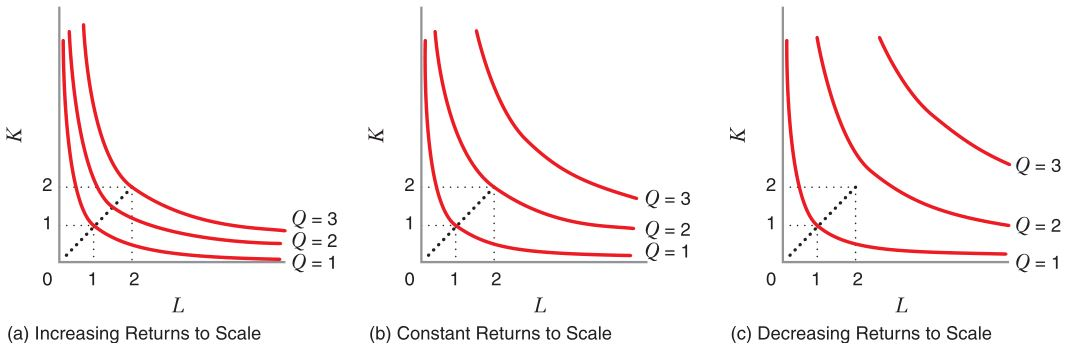
\includegraphics[width = \linewidth]{figures/fig6_18.jpg}
  \end{figure}
\end{frame}

\begin{frame}{Returns to Scale}
  Why are returns to scale important? Suppose a firm exhibits increasing returns to scale.

  \begin{itemize}
    \item Then they could produce more output than two firms that are each half the size of the single firm.

    \item Or they could produce the same amount of output at a \textit{lower cost per unit}.
  \end{itemize}

  \bigskip
  This can mean that a market is more efficiently served by one large firm, rather than two smaller ones.

  \begin{itemize}
    \item This is why governments may often allow certain monopolies to operate (such as utility companies).
  \end{itemize}
\end{frame}

\begin{frame}
  \bgCranberry{Try It Yourself}
  
  \bigskip
  Suppose a firm has the following production function: $Q(K,L) = 4K^{\frac{1}{2}}L^{\frac{1}{2}}$. Does this production function exhibit increasing, decreasing, or constant returns to scale?
\end{frame}

\begin{frame}
  \bgCranberry{Try It Yourself}

  \bigskip
  Which of the following production functions exhibits decreasing returns to scale?

  \bigskip
  \begin{enumerate}[A)]
    \item $Q(K,L) = 2K+3L$
    \item $Q(K,L) = \sqrt{K}L$
    \item $Q(K,L) = K^{1/3}L^{1/3}$
    \item $Q(K,L) = 2\sqrt{K} + \sqrt{L}$
  \end{enumerate}
\end{frame}

\begin{frame}{Returns to Scale vs. Marginal Returns}
  It's important to understand the distinction between returns to scale and marginal returns.
  
  \bigskip
  \begin{itemize}
    \item Returns to scale pertain to the impact of an increase in \textit{all input quantities} simulaneously.

    \item Marginal returns deal with increasing the quantity of \textit{a single input}.
  \end{itemize}

  \pause\bigskip
  A firm can have diminishing marginal returns to it's inputs, but still experience constant (or even increasing) returns to scale.
  
  \begin{itemize}
    \item Doubling the number lawnmowers doesn't increase output without additional workers. But doubling the number of both could potentially double output.
  \end{itemize}
\end{frame}

\begin{frame}{Returns to Scale vs. Marginal Returns}
  This graph illustrates a production function with diminishing marginal product of labor (see points A, B, and C), but constant returns to scale.

  \begin{figure}
    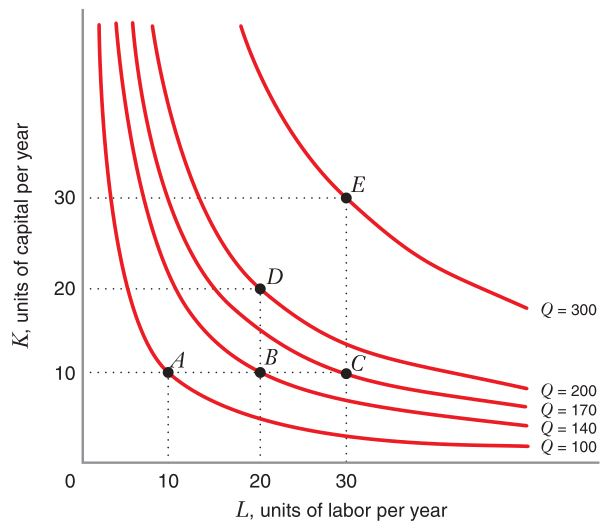
\includegraphics[width=0.6\linewidth]{figures/fig6_19.jpg}
  \end{figure}
\end{frame}

\begin{frame}{Technological Progress}
  Until now, we've treated a firm's production function as if it were fixed
  
  \bigskip
  \begin{itemize}
    \item The quantity of inputs could vary, but the relationship between inputs and output did not change.
  \end{itemize}

  \bigskip
  But \textbf{technological progress} can allow a firm to produce more output from a given combination of inputs.

  \begin{itemize}
    \item New production techniques can be discovered, worker's can learn new techniques, etc.

    \item This technological progress can shift the production function.
  \end{itemize}
\end{frame}

\begin{frame}{Technological Progress}
  As firms devise ways to produce the same amount of output with a lower quantity of inputs, the isoquants of a production function shift inward.
  
  \bigskip
  Technological progress can be broadly classified into three categories:
  \begin{enumerate}
    \item Neutral technological progress
    
    \item Labor-saving technological progress
    
    \item Capital-saving technological progress
  \end{enumerate}
\end{frame}
  
\begin{frame}{Technological Progress}
  \textbf{Neutral technological progress} refers to inward shifts in the isoquant (so that a given quantity of output can be produced using fewer inputs), where the $MRTS_{L,K}$ is unchanged.
  
  \bigskip
  \begin{itemize}
    \item Both factors become more productive in equal proportions.
  \end{itemize}
\end{frame}

\begin{frame}
  With \textbf{netural technological progress}, the same quantity of output can be produced with fewer inputs, but the $MRTS_{L,K}$ remains the same.

  \bigskip
  \begin{figure}
    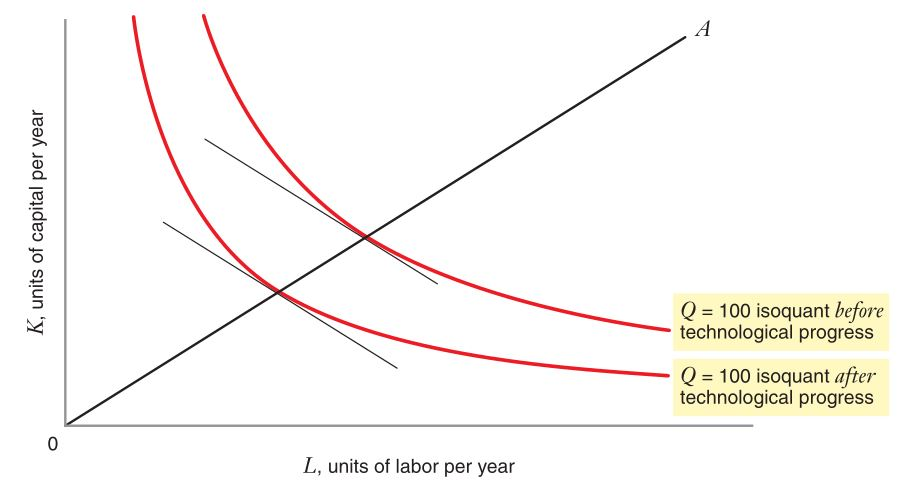
\includegraphics[width=0.8\linewidth]{figures/fig6_20.jpg}
  \end{figure}
\end{frame}

\begin{frame}{Technological Progress}
  With \textbf{labor-saving} (or \textbf{capital-biased}) technological progress, capital becomes more productive relative to labor.

  \bigskip
  \begin{itemize}
    \item That means that $MP_K$ increases proportionally more than $MP_L$, so the $MRTS_{L,K}$ decreases.
  \end{itemize}
\end{frame}

\begin{frame}
  With \textbf{labor-saving technological progress}, the same quantity of output can be produced with fewer inputs, and the $MRTS_{L,K}$ decreases.

  \bigskip
  \begin{figure}
    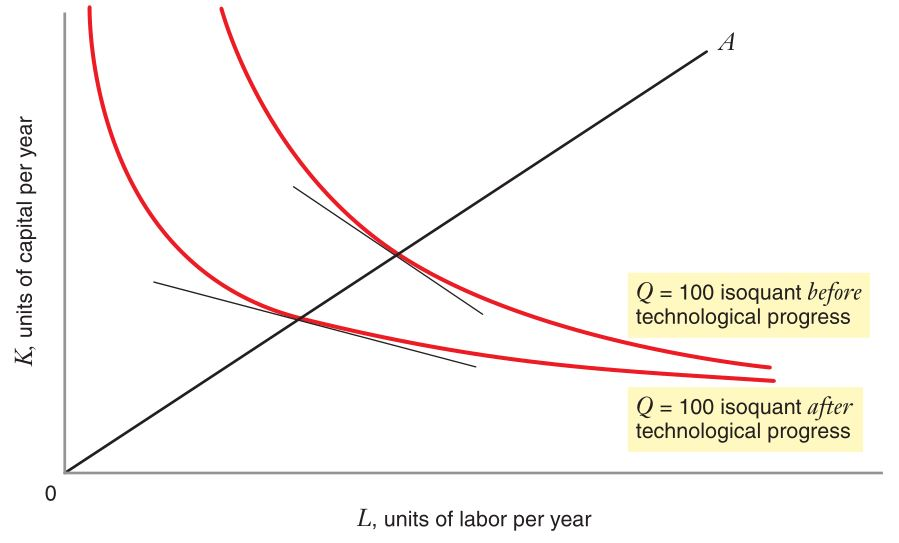
\includegraphics[width=0.8\linewidth]{figures/fig6_21.jpg}
  \end{figure}
\end{frame}

\begin{frame}{Technological Progress}
  With \textbf{capital-saving} (or \textbf{labor-biased}) technological progress, labor becomes more productive relative to capital.
  
  \bigskip
  \begin{itemize}
    \item $MP_L$ increases proportionally more than $MP_K$, so the $MRTS_{L,K}$ increases.
  \end{itemize}
\end{frame}

\begin{frame}
  With \textbf{capital-saving technological progress}, the same quantity of output can be produced with fewer inputs, and the $MRTS_{L,K}$ increases.

  \bigskip
  \begin{figure}
    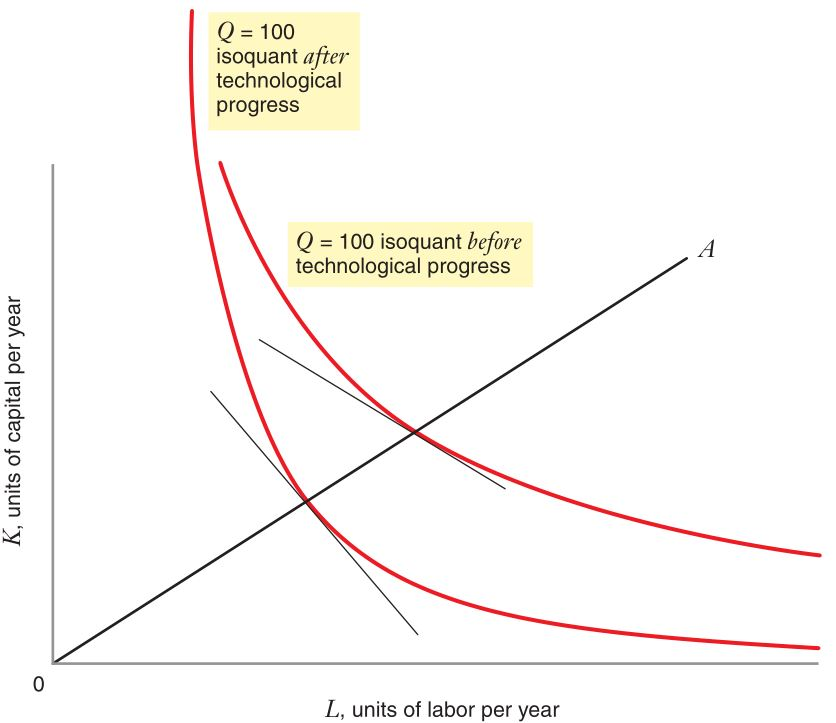
\includegraphics[width=0.6\linewidth]{figures/fig6_22.jpg}
  \end{figure}
\end{frame}

\begin{frame}
  \bgCranberry{Try It Yourself}
  
  \bigskip
  Suppose that a firm initially has the production function $Q(K,L) = K+L$. After a period of time, the production function changes to $Q(K,L) = 3K+2L$. What type of technological progress does this represent?
\end{frame}

\end{document}
